\newpage
\section{Architektura}

Przepływ danych między kolejnymi detektorami wykorzystywanymi w~aplikacji został przedstawiony na diagramie \ref{fig:architecture}.

\begin{figure}[!h]
    \begin{center}
        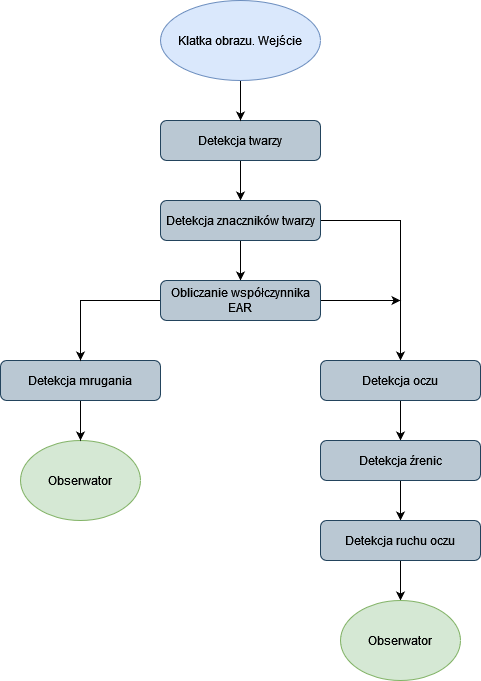
\includegraphics[scale=0.5]{img/architecture.png}
        \caption{Diagram przepływu detekcji i danych.}
        \label{fig:architecture}
    \end{center}
\end{figure}



\subsection{Wzorce projektowe}

W ramach implementacji projektu zostały zastosowane dwa istotne dla działania aplikacji wzorce projektowe: wstrzykiwania zależności oraz obserwator. 


\subsubsection{Wstrzykiwanie zależności}

W myśl tego rozwiązania komponenty klasy nie są tworzone bezpośrednio w~niej, lecz poza nią, a~następnie za pomocą metody (ang. setter injection) lub konstruktora (ang.~constructor injection) są \textit{wstrzykiwane} i~przypisywane do własności tej klasy. 

\par

Zastosowanie tego wzorca pozwala zmniejszyć sprzężenia między klasami, co jest dobrą praktyką programowania. 




\paragraph{Przykład użycia} Istnieje klasa detektora twarzy, która podczas swojego działania wykorzystuje algorytm detekcji, którego instancja jest przechowywana w~polu tej klasy.

\par

Przykładowo kod tej klasy gdy instancja algorytmu detekcji tworzona jest w~jej konstruktorze może wyglądać tak:

\vspace{5mm}

\begin{addmargin}[10mm]{0mm}
\begin{lstlisting}[
    language=Java,
    numbers=left,
    firstnumber=1,
    caption={Przykład klasy bez użycia wzorca wstrzykiwania zależności},
    aboveskip=0pt
]
class FaceDetector {
    private final FaceDetectionAlgorithm detectionAlgorithm;
    
    public FaceDetector() {
        detectionAlgorithm = new FaceDetectionAlgorithm();
    }
}
\end{lstlisting}
\end{addmargin}

\vspace{5mm}

Natomiast, kod w~przypadku gdy wykorzystany jest wzorzec wstrzykiwania zależności, a~instancja algorytmu detekcji tworzona jest poza nią może wyglądać następująco:

\vspace{5mm}

\begin{addmargin}[10mm]{0mm}
\begin{lstlisting}[
    language=Java,
    numbers=left,
    firstnumber=1,
    caption={Przykład klasy z użyciem wzorca wstrzykiwania zależności},
    aboveskip=0pt
]
class FaceDetector {
    private final FaceDetectionAlgorithm detectionAlgorithm;
    
    public FaceDetector(FaceDetectionAlgorithm detectionAlgorithm) {
        this.detectionAlgorithm = detectionAlgorithm;
    }
}
\end{lstlisting}
\end{addmargin}


\vspace{5mm}


\paragraph{Wykorzystanie w projekcie}

W projekcie pracy dyplomowej wzorzec wstrzykiwania zależności występuje w~następujących detektorach:

\begin{itemize}
    \item Twarzy
    \item Znaczników
    \item Oczu
    \item Źrenic
\end{itemize}
    
W wypadku tych klas wstrzykiwane są do nich wybrane metody detekcji poszczególnych części twarzy. Dzięki zastosowaniu takiego rozwiązania istnieje łatwa możliwość zmiany algorytmu bez potrzeby ingerowania i~dostosowania całego systemu, ponieważ implementują one interfejs z~metodą, która wywołuje dany detektor. 
    
    
    
\subsubsection{Obserwator}

Polega na połączeniu klas w~relacje obserwowany-obserwatorzy. Ten pierwszy przechowując odwołania do wszystkich obiektów może je poinformować o~zmianach własnego stanu.

\par

Zaletą stosowania tego rozwiązania są \textit{luźne powiązania} między obiektem obserwowanym, a~obserwatorem. Dodatkowo pozwala on na dynamiczne zmienianie zależności między tymi obiektami w~czasie wykonywania programu. 


\paragraph{Wykorzystanie w projekcie} W~stworzonej aplikacji wzorzec obserwatora został zastosowany w~przypadku wykrywania detekcji ruchu oczu i~mrugania. Gdy zostanie stwierdzone wystąpienie któregoś z~tych zdarzeń odpowiednia klasa wysyła informację o~tym do obserwatorów. Mogą one wtedy odpowiednio zareagować na te zmiany. Pozwala to na łatwe dodawanie nowych komponentów, które swoje działanie uzależniają od mrugania i~ruszania oczami przez użytkownika. 